\subsection*{Preliminaries}
%--------------------------------------------------------------------------------------------------
%\begin{frame}[t]
%    \frametitle{Preliminaries}
%    \framesubtitle{Vision}
%    One way we process information. 
%    Arguably the most important sense, in terms of energy consumption \cite{phelps1981metabolic},
%    also leading to evolution \cite{mattson2014superior}\\\pause
%    \begin{columns}
%        \column[T]{0.5\textwidth}
%        Approached on fields such as:
%        \begin{itemize}
%            \item Medicine.
%            \item Physics.
%            \item Psychology.
%        \end{itemize}
%        \column[T]{0.5\textwidth}
%        \begin{center}
%            \begin{tikzpicture}
%                \node[] at (0,0) (img_brain) 
%                    {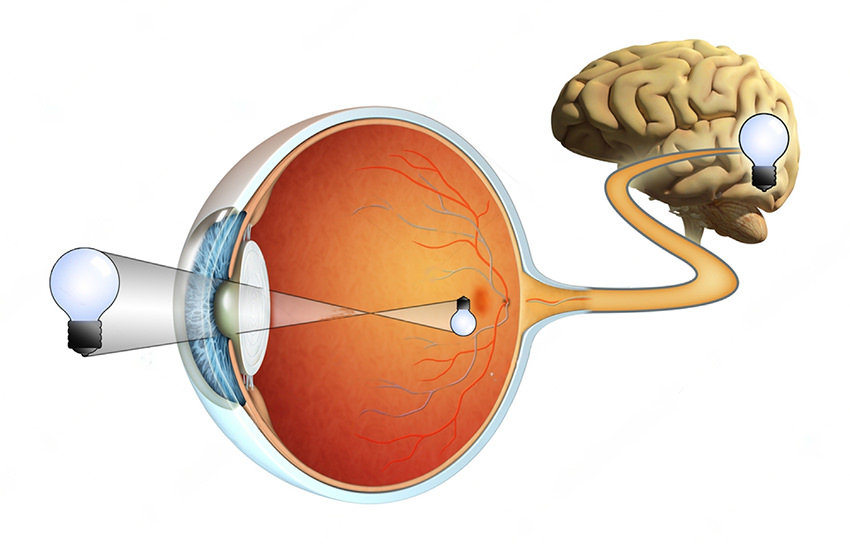
\includegraphics[scale=0.1]{fig/rel/common/img/brain_n_vision.jpg}};
%                \node[] at (img_brain.south east) (img_newton) 
%                    {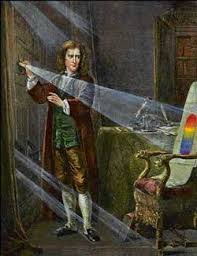
\includegraphics[scale=0.25]{fig/rel/common/img/newton_color.jpeg}};
%                \node[] at (img_newton.south west) (img_gestalt) 
%                    {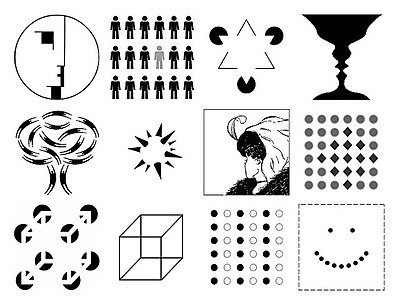
\includegraphics[scale=0.175]{fig/rel/common/img/gestalt.jpg}};
%            \end{tikzpicture}
%        \end{center}
%    \end{columns}
%\end{frame}
%--------------------------------------------------------------------------------------------------
%\begin{frame}[t]
%    \frametitle{Preliminaries}
%    \framesubtitle{David Marr's approach}
%    \begin{columns}[t]
%        \column{0.5\textwidth}
%        \begin{center}
%            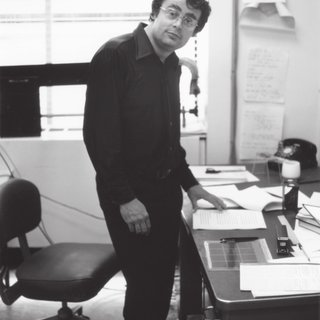
\includegraphics[width=0.8\textwidth]{fig/rel/common/img/Marr.jpg}    
%        \end{center}
%        \column{0.5\textwidth}
%        Addressing vision on three levels:
%        \begin{itemize}
%            \item Algorithmic.
%            \item Implementation.
%            \item Computational.
%            \begin{itemize}
%                \item Three fundamental tasks. \cite{malik2016three}
%            \end{itemize}
%        \end{itemize}
%        \pause
%        \vspace{20pt}
%        \textbf{Computer Vision focuses on the last level.}
%        
%    \end{columns}
%    
%\end{frame}
%--------------------------------------------------------------------------------------------------
%\begin{frame}[t]
%    \frametitle{Preliminaries}
%    \framesubtitle{Desiredata of Interpretability Study \cite{mythos_interp}}
%    \small
%    \begin{columns}[c]
%        \column[T]{0.4\textwidth}      
%            We ask  questions regarding \emph{black box models}.
%            \begin{itemize}
%                    \item How does it work?
%                    \item How safe is it?
%                    \item Who is accountable for it?
%                    \item Who benefits from it?
%                    \item Who uses it?
%            \end{itemize}
%        \column[T]{0.6\textwidth}
%        \pause
%        \begin{center}
%                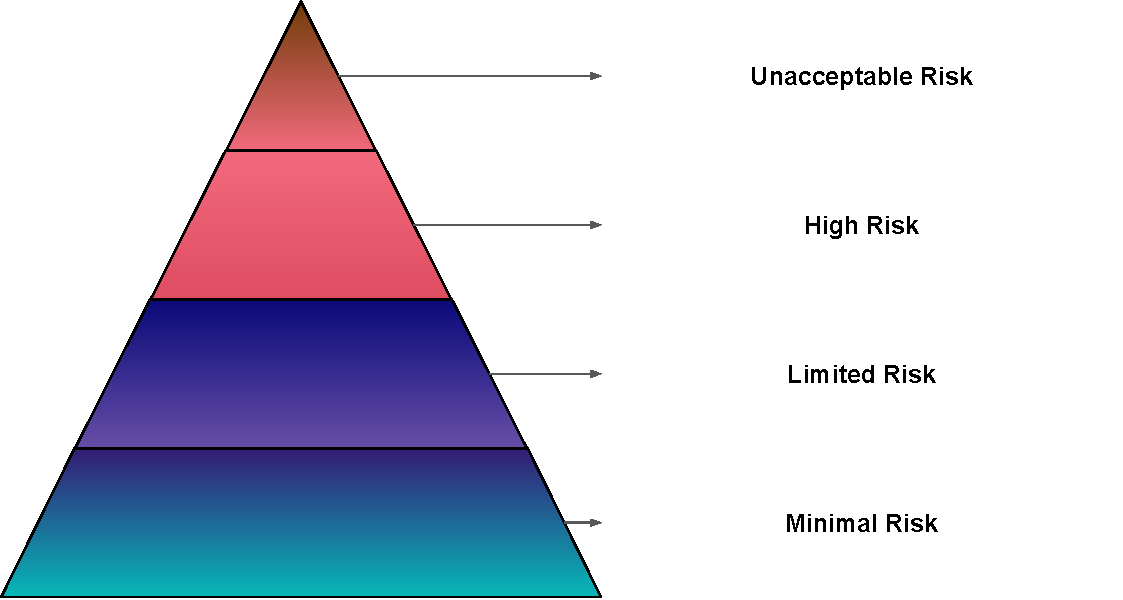
\includegraphics[width=\textwidth]{fig/rel/common/img/AI_act_pyramid.pdf}      
%                \small Regulation planned with the European AI act\cite{madiega2021artificial}
%        \end{center}
%        \vspace{10pt}
%        \textbf{Accepted AI systems within society must answer this.}
%
%    \end{columns}
%\end{frame}